\documentclass[a4paper,11pt]{article}

\usepackage[T1]{fontenc}
\usepackage[utf8]{inputenc}
\usepackage{graphicx}
\usepackage{xcolor}

\renewcommand\familydefault{\sfdefault}
\usepackage{tgheros}
\usepackage[defaultmono]{droidmono}

\usepackage{amsmath,amssymb,amsthm,textcomp}
\usepackage{enumerate}
\usepackage{multicol}
\usepackage{tikz}
\usepackage{graphics}
\usepackage{lstlinebgrd}
\usepackage{color}
\usepackage{geometry}
\geometry{total={210mm,297mm},
left=25mm,right=25mm,%
bindingoffset=0mm, top=20mm,bottom=20mm}


\linespread{1.3}

\newcommand{\linia}{\rule{\linewidth}{0.5pt}}

\newtheoremstyle{mytheor}
    {1ex}{1ex}{\normalfont}{0pt}{\scshape}{.}{1ex}
    {{\thmname{#1 }}{\thmnumber{#2}}{\thmnote{ (#3)}}}

\theoremstyle{mytheor}
\newtheorem{defi}{Definition}

% my own titles
\makeatletter
\renewcommand{\maketitle}{
\begin{center}
\vspace{2ex}
{\huge \textsc{\@title}}
\vspace{1ex}
\\
\linia\\
\@author \hfill \@date
\vspace{4ex}
\end{center}
}
\makeatother
%%%

% custom footers and headers
\usepackage{fancyhdr}
\pagestyle{fancy}
\lhead{Page \thepage}
\chead{}
\rhead{Steven Seppala}
\lfoot{Homework assignment \textnumero{} 3}
\cfoot{Operating Systems}
\rfoot{ECE 437}
\renewcommand{\headrulewidth}{0pt}
\renewcommand{\footrulewidth}{0pt}
%

% code listing settings
\usepackage{listings}
\lstset{
    language=[ANSI]C,
    basicstyle=\ttfamily\small,
    aboveskip={1.0\baselineskip},
    belowskip={1.0\baselineskip},
    columns=fixed,
    extendedchars=true,
    breaklines=true,
    tabsize=4,
    prebreak=\raisebox{0ex}[0ex][0ex]{\ensuremath{\hookleftarrow}},
    frame=lines,
    showtabs=false,
    showspaces=false,
    showstringspaces=false,
    keywordstyle=\color[rgb]{0.627,0.126,0.941},
    commentstyle=\color[rgb]{0.133,0.545,0.133},
    stringstyle=\color[rgb]{01,0,0},
    numbers=left,
    numberstyle=\small,
    stepnumber=1,
    numbersep=10pt,
    captionpos=t,
    escapeinside={\%*}{*)}
}
	\definecolor{dkgreen}{rgb}{0,0.8,0}
	\definecolor{gray}{rgb}{0.5,0.5,0.5}
	\definecolor{mauve}{rgb}{0.58,0,0.82}

%%%----------%%%----------%%%----------%%%----------%%%
%%%----------Document begins right below this-------%%%
%%%----------%%%----------%%%----------%%%----------%%%
\begin{document}

\title{Homework Assignment \textnumero{} 3}

\author{Steven Seppala}

\date{22 November 2014}

\maketitle

\begin{center} \section*{Homework assignment 3} \end{center}

\begin{enumerate}
\item {Problem 8.11} 
    \par 
    \begin{enumerate}
    \item First-fit\par
        P1 => Mem(1) with 185 left\\
        P2 => Mem(2) with 100 left \\
        P3 => Mem(5) with 392 left\\
        P4 => Mem(3) with 150 left\\
        P5 => Mem(5)\\
    \item Best-fit \par
        P1 => Mem(6) with 10 left\\
        P2 => Mem(2) with 100 left\\
        P3 => Mem(5) with 392 left\\
        P4 => Mem(4) with 0 left\\
        P5 => Mem(5)\\
    \item Worst-fit \par
        P1 => Mem(4)\\
        P2 => Mem(4)\\
        P3 => Mem(2)\\
        P4 => Mem(1)\\
        P5 => Fragmentation as it waits for Mem(2) or Mem(4)\\
    \end{enumerate}
\item {Problem 8.25}
    \par 
    A) $2* 50$ ns = $100$ ns \\
    B) $2 + (.75 * 50) + (.25 * 100) =$ $64.5$ ns\\ 
\pagebreak
\item{Problem 9.30}
    \begin{enumerate}
    \item Define a page-replacement algorithm \par
        \begin{enumerate}
        \item Starting counter value : 0
        \item Counters are increase whenever a new page is associated with that frame
        \item Counters are decreased whenever one of the pages of 
                the frame is no longer needed
        \item The page replacement is selected by breaking FIFO 
                for tie breaking and finding frame with the smallest counter.
        \end{enumerate}
    \item Page faults for the string.  = 13 \par
        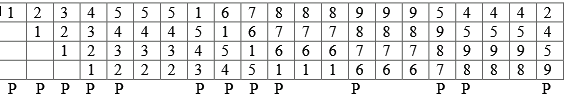
\includegraphics[width=1\textwidth]{930_PB.png}
    \item Minimum possible page faults = 11\par
        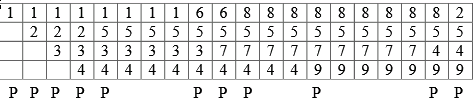
\includegraphics[width=1\textwidth]{930_PC.png}
    \end{enumerate}
\item{Problem 9.35}
    The 240-byte request is assigned a 256-byte segment\\ 
    The 120-byte request is assigned a 128-byte segment\\
    The 60-byte request is assigned a 64-byte segment \\
    The 130-byte request is assigned a 256-byte segment.\\
    After the allocation, the following segment sizes are available:\\
    64-bytes, 256-bytes, 1K, 2K, 4K, 8K, 16K, 32K, 64K, 128K, 256K, \& 512K.\\
    
    After the releases of memory, the only segment in use would be a 256-byte segment containing 130 bytes of data. \\
    The following segments will be free: \\
    256 bytes, 512 bytes, 1K, 2K, 4K, 8K, 16K, 32K, 64K, 128K, 256K, \& 512K.

    \pagebreak

\item{Problem 12.9} \par
    \begin{enumerate}
    \item All extens are of the same size \par 
        The amount of free space needed for a file must be known in advance, pre-allocation might be inefficient; a file the grows over time must have enough space allocated for its final size. Regardless of how often the file is used. This may invoke internal fragmentation. \\
        The advantage is foe sequential access; the file system remembers the disk address of the block last referenced and thus can read the next block quickly.
    \item Extents can be of any size and are allocated dynamically.\\
        Dynamic allocation involves how to satisfy a request of variable size from a list of free holes. This advantage means that there will be no internal fragmentation. But the first fit and best fit methods for selecting a free hole suffers from external fragmentation.
    \item Extents can be of a few predetermined sizes. \\
        External fragmentation becomes a problem when the largest contiguous chunks are unable to handle a request; storage is fragmented into holes too small to handle the data, depending on the file and disk size.
    \end{enumerate}
    
\item{Problem 12.11} \par
    The advantage is that while accessing a block that is stored at the middle of a file, its location can be determined by chasing the pointers stored in the FAT as opposed to accessing all of the individual blocks of the file in a sequential manner to find the pointer to the target block. Typically, most of the FAT can be cached in memory and therefore the pointers can be determined with just memory accesses instead of having to access the disk blocks 
    
\item{Problem 10.11}
    \begin{enumerate}
        \item[(a)]FCFS {\color{black}The schedule is 2150, 2069, 1212, 2296, 2800, 544, 1618, 356, 1523, 4965, 3681. The total distance is 13011.}
        \item[(b)]SSTF {\color{black}The schedule is 2150, 2069, 2296, 2800, 3681, 4965, 1618, 1523, 1212, 544, 356. The total distance is 7586.}
        \item[(c)]SCAN {\color{black}The schedule is 2150, 2069, 1618, 1523, 1212, 544, 356, 0, 2296, 2800, 3681, 4965. The total distance is 7115.}
        \item[(d)]LOOK {\color{black}The schedule is 2150, 2069, 1618, 1523, 1212, 544, 356, 2296, 2800, 3681, 4965. The total distance is 6403.}
        \item[(e)]C-SCAN {\color{black}The schedule is 2150, 2296, 2800, 3681, 4965, 4999, 0, 356, 544, 1212, 1523, 1618, 2069. The total distance is 9917.}
        \item[(f)]C-LOOK {\color{black}The schedule is 2150, 2296, 2800, 3681, 4965, 356, 544, 1212, 1523, 1618, 2069. The total distance is 9137.}
\end{enumerate}


\pagebreak

\item{Problem 10.17}
    \begin{enumerate}
    \item[A] a) A write of one block of data requires the following: read
of the parity block, read of the old data stored in the target block,
computation of the new parity based on the differences between the
new and old contents of the target block, and write of the parity block
and the target block. 
    \item[B]
    Assume that the seven contiguous blocks begin
at a four-block boundary. A write of seven contiguous blocks of data
could be performed by writing the seven contiguous blocks, writing the
parity block of the first four blocks, reading the eight block, computing
the parity for the next set of four blocks and writing the corresponding
parity block onto disk.
    \end{enumerate}
    
\item{Problem 15.3} \par
    When a user creates a password, the system generates a
random number (which is the salt) and appends it to the user-provided
password, encrypts the resulting string and stores the encrypted result
and the salt in the password file. When a password check is to be
made, the password presented by the user is first concatenated with
the salt and then encrypted before checking for equality with the stored
password. Since the salt is different for different users, a password
cracker cannot check a single candidate password, encrypt it, and check
it against all of the encrypted passwords simultaneously

\item{Problem 15.13} \par
    It means that the message is encrypted
using the public key and then decrypted using the private key. This
scheme is not sufficient to guarantee authentication since any entity
can obtain the public keys and therefore could have fabricated the
message. However, the only entity that can decrypt the message is the
entity that owns the private key, which guarantees that the message is
a secret message from the sender to the entity owning the private key;
no other entity can decrypt the contents of the message.
    
    
\end{enumerate}
\end{document}